\chapter{परमाण्वीय कक्षक: आकृतियाँ, ऊर्जाएँ और आकार}\label{ch:b2:atomic-orbitals}

हाइड्रोजन परमाणु का कोई किनारा नहीं होता: उसका इलेक्ट्रॉन नाभिक से किसी भी दूरी पर
मिल सकता है, ऐसी प्रायिकता के साथ जो तेज़ी से घटती है परंतु कभी शून्य तक नहीं
पहुँचती। फिर भी परमाणुओं के आकार होते हैं, और सोडियम परमाणु क्लोरीन परमाणु से
लगभग दुगुना चौड़ा है, यद्यपि उसमें कम इलेक्ट्रॉन हैं। प्रथम वर्ष के खंड ने
इलेक्ट्रॉन की अवस्थाओं को तीन क्वांटम संख्याओं से नाम दिया था; यहाँ उनमें से हर एक
स्थिति का एक फलन बन जाती है, जिसकी एक आकृति, नोड, चिह्न और एक आकार होता है, और नियमों का एक सरल
समुच्चय उन्हें किसी भी परमाणु के लिए कक्षक ऊर्जाओं में बदल देता है। यही आकृतियाँ और चिह्न
हैं जिन्हें अगले चार अध्याय आण्विक कक्षकों में संयोजित करते हैं।

\begin{recall}
प्रथम वर्ष का खंड: क्वांटम संख्याएँ $n$, $l$, $m_l$, $m_s$; अवस्थाओं $(n, l, m_l)$ के रूप में
परमाण्वीय कक्षक; कोश और उपकोश; आवरण और प्रभावी नाभिकीय
आवेश (गुणात्मक रूप से); इलेक्ट्रॉनिक विन्यास; हाइड्रोजन के स्तर,
$-E_R/n^2$, जहाँ $E_R = \qty{13.6}{eV}$। भौतिकी से: \omterm{def:b2:atomic-orbitals:wavefunction}{तरंग फलन}, जिसके
मापांक का वर्ग \omterm{def:b2:atomic-orbitals:wavefunction}{प्रायिकता घनत्व} है।
\end{recall}

\section{हाइड्रोजन परमाणु के तरंग फलन}

\begin{definition}[तरंग फलन]\label{def:b2:atomic-orbitals:wavefunction}
इलेक्ट्रॉन की अवस्था का वर्णन एक \emph{तरंग फलन}\index{तरंग फलन}
$\psi(x, y, z)$ से होता है; $|\psi|^2$ उसका \emph{प्रायिकता घनत्व}\index{प्रायिकता घनत्व} है:
किसी बिंदु के चारों ओर छोटे आयतन $dV$ में इलेक्ट्रॉन के मिलने की प्रायिकता
$|\psi|^2\,dV$ है, और पूरे आकाश पर $\int|\psi|^2\,dV = 1$ (फलन
प्रसामान्यीकृत है)। परमाण्वीय कक्षक किसी परमाणु में एक इलेक्ट्रॉन का
तरंग फलन है।
\end{definition}

\begin{definition}[त्रिज्य और कोणीय भाग]\label{def:b2:atomic-orbitals:radial-angular}
नाभिक के परितः गोलीय निर्देशांकों $(r, \theta, \varphi)$ में
हाइड्रोजन-सदृश परमाणु के कक्षक $\psi_{nlm}(r, \theta, \varphi) = R_{nl}(r)\,
Y_{lm}(\theta, \varphi)$ के रूप में गुणनखंडित होते हैं: \emph{त्रिज्य भाग}\index{त्रिज्य भाग} $R_{nl}$
$n$ और $l$ पर निर्भर करता है, \emph{कोणीय भाग}\index{कोणीय भाग} $Y_{lm}$ केवल $l$ और
$m_l$ पर।
\end{definition}

\begin{theorem}[हाइड्रोजन-सदृश कक्षक]\label{thm:b2:atomic-orbitals:hydrogen}
नाभिकीय आवेश $Ze$ वाले एक-इलेक्ट्रॉन परमाणु के लिए, $\rho = Zr/a_0$ और बोर त्रिज्या $a_0 =
\qty{52.9}{pm}$ के साथ, $n \leq 3$ के लिए \omterm{def:b2:atomic-orbitals:radial-angular}{त्रिज्य भाग},
$(Z/a_0)^{3/2}$ की इकाइयों में, ये हैं:
\[
\begin{array}{ll}
  R_{1s} = 2\,\mathrm e^{-\rho} &
  R_{2s} = \dfrac{1}{2\sqrt2}\,(2 - \rho)\,\mathrm e^{-\rho/2} \\[2ex]
  R_{2p} = \dfrac{1}{2\sqrt6}\,\rho\,\mathrm e^{-\rho/2} &
  R_{3s} = \dfrac{2}{81\sqrt3}\,(27 - 18\rho + 2\rho^2)\,\mathrm e^{-\rho/3} \\[2ex]
  R_{3p} = \dfrac{4}{81\sqrt6}\,(6\rho - \rho^2)\,\mathrm e^{-\rho/3} &
  R_{3d} = \dfrac{4}{81\sqrt{30}}\,\rho^2\,\mathrm e^{-\rho/3}
\end{array}
\]
और वास्तविक \omterm{def:b2:atomic-orbitals:radial-angular}{कोणीय भाग} $Y_s = 1/\sqrt{4\pi}$; $Y_{p_x}, Y_{p_y}, Y_{p_z} =
\sqrt{3/(4\pi)}\,(x, y, z)/r$; $Y_{d_{xy}} = \sqrt{15/(4\pi)}\,xy/r^2$ (और इसी प्रकार
$xz$, $yz$), $Y_{d_{x^2-y^2}} = \sqrt{15/(16\pi)}\,(x^2 - y^2)/r^2$, $Y_{d_{z^2}} =
\sqrt{5/(16\pi)}\,(3z^2 - r^2)/r^2$ हैं। उनकी ऊर्जाएँ $E_n = -Z^2E_R/n^2$ हैं।
% ledger: const:a0, const:RyhcEV
\end{theorem}

\admitted

ये फलन एक इलेक्ट्रॉन और एक नाभिक के लिए श्रोडिंगर समीकरण के हल हैं,
जो तृतीय वर्ष के खंड में प्राप्त किए गए हैं। वास्तविक $p$ और $d$ फलन $m_l$ द्वारा
अंकित सम्मिश्र फलनों के संयोजन हैं; वे अक्षों के अनुदिश इंगित करते हैं और
आबंध बनाने में यही प्रयुक्त होते हैं।

\begin{omfigure}
\begin{minipage}[t]{0.27\linewidth}\vspace{0pt}
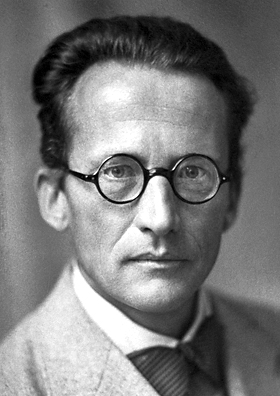
\includegraphics[width=\linewidth]{images/book3/schrodinger.jpg}
\end{minipage}\hfill
\begin{minipage}[t]{0.69\linewidth}\vspace{0pt}
{\small एर्विन श्रोडिंगर, जिन्होंने 1926 में वह तरंग समीकरण लिखा जिसके
हाइड्रोजन परमाणु के लिए हल इस अध्याय के कक्षक हैं, और जिन्होंने उनसे वे
ऊर्जा स्तर पुनः प्राप्त किए जिनकी बोर ने अभिधारणा की थी। उन्हें 1933 में भौतिकी का नोबेल
पुरस्कार साझा रूप से मिला। (छायाचित्र: नोबेल फ़ाउंडेशन, सार्वजनिक अधिकार-क्षेत्र,
विकिमीडिया कॉमन्स।)}
\end{minipage}
\end{omfigure}

\section{त्रिज्य भाग}

त्रिज्याओं $r$ और $r +
dr$ वाले गोलों के बीच इलेक्ट्रॉन के मिलने की प्रायिकता $|\psi|^2$ है, जिसे $4\pi r^2\,dr$ आयतन वाले कोश पर समाकलित किया गया हो;
किसी भी कक्षक के लिए, कोणों पर समाकलन कर लेने के बाद, यह $r^2R^2\,dr$ है।

\begin{definition}[त्रिज्य वितरण]\label{def:b2:atomic-orbitals:radial-distribution}
किसी कक्षक का \emph{त्रिज्य वितरण फलन}\index{त्रिज्य वितरण फलन}
$P(r) = r^2R_{nl}(r)^2$ है: $P(r)\,dr$ वह प्रायिकता है कि
इलेक्ट्रॉन नाभिक से $r$ और $r + dr$ के बीच हो। \emph{सर्वाधिक संभाव्य
त्रिज्या}\index{सर्वाधिक संभाव्य त्रिज्या} उसके सबसे बड़े अधिकतम पर $r$ का मान है।
\end{definition}

\begin{proposition}[1s का प्रसामान्यीकरण]\label{prop:b2:atomic-orbitals:normalised}
$\int_0^\infty P_{1s}(r)\,dr = 1$.
\end{proposition}

\begin{proof}\emergencystretch=3em
$Z = 1$ के साथ, और $r$ को $a_0$ की इकाइयों में लेकर, $P_{1s} = 4r^2\mathrm e^{-2r}$। दो बार खंडशः समाकलन से
$\int_0^\infty r^2\mathrm e^{-2r}\,dr = \frac22\int_0^\infty r\,\mathrm e^{-2r}\,dr =
\frac12\int_0^\infty\mathrm e^{-2r}\,dr = \frac14$, और $4 \times \frac14 = 1$।
\end{proof}

\begin{proposition}[सर्वाधिक संभाव्य त्रिज्या]\label{prop:b2:atomic-orbitals:most-probable}
1s कक्षक के लिए \omterm{def:b2:atomic-orbitals:radial-distribution}{सर्वाधिक संभाव्य त्रिज्या} $a_0/Z$ है। $l =
n - 1$ वाले कक्षक (1s, 2p, 3d, \dots) के लिए यह $n^2a_0/Z$ है।
\end{proposition}

\begin{proof}
$l = n - 1$ के लिए \omterm{def:b2:atomic-orbitals:radial-angular}{त्रिज्य भाग} में कोई नोड नहीं होता: $R \propto \rho^{n-1}\mathrm e^{-\rho/n}$,
अतः $P \propto \rho^{2n}\mathrm e^{-2\rho/n}$ और $d\ln P/d\rho = 2n/\rho - 2/n$, जो
$\rho = n^2$ के लिए शून्य है, अर्थात् $r = n^2a_0/Z$। $n = 1$ के साथ $r = a_0/Z$।
\end{proof}

\begin{proposition}[1s की माध्य त्रिज्या]\label{prop:b2:atomic-orbitals:mean-radius}
नाभिक से 1s इलेक्ट्रॉन की माध्य दूरी $\langle r\rangle = 3a_0/(2Z)$ है,
जो उसकी \omterm{def:b2:atomic-orbitals:radial-distribution}{सर्वाधिक संभाव्य त्रिज्या} से बड़ी है।
\end{proposition}

\begin{proof}
$Z = 1$ के साथ: $\langle r\rangle = \int_0^\infty r\,P(r)\,dr = 4\int_0^\infty r^3\mathrm e^{-2r}
\,dr = 4 \times 3!/2^4 = 3/2$। वितरण की बड़े $r$ पर लंबी पूँछ है,
जो माध्य को अधिकतम से आगे खींच लेती है।
\end{proof}

\begin{definition}[नोड]\label{def:b2:atomic-orbitals:node}
किसी कक्षक की \emph{नोडीय सतह}\index{नोडीय सतह} वह सतह है जिस पर
\omterm{def:b2:atomic-orbitals:wavefunction}{तरंग फलन} शून्य होता है और चिह्न बदलता है। यह \emph{त्रिज्य नोड}\index{त्रिज्य नोड}
(एक गोला) है जब \omterm{def:b2:atomic-orbitals:radial-angular}{त्रिज्य भाग} लुप्त होता है, और \emph{कोणीय
नोड}\index{कोणीय नोड} (नाभिक से होकर जाने वाला एक तल या शंकु) जब \omterm{def:b2:atomic-orbitals:radial-angular}{कोणीय भाग}
लुप्त होता है।
\end{definition}

\begin{proposition}[नोडों की गिनती]\label{prop:b2:atomic-orbitals:nodes}
कक्षक $(n, l)$ के $n - l - 1$ \omterm{def:b2:atomic-orbitals:node}{त्रिज्य नोड} और $l$ \omterm{def:b2:atomic-orbitals:node}{कोणीय नोड} होते हैं, कुल
$n - 1$।
\end{proposition}

\begin{proof}
\cref{thm:b2:atomic-orbitals:hydrogen} के फलनों पर: $R_{2s}$
$\rho = 2$ पर शून्य होता है, $R_{3s}$, $2\rho^2 - 18\rho + 27$ के दोनों मूलों ($\rho = 1.90$ और $7.10$) पर,
$R_{3p}$, $\rho = 6$ पर; $R_{1s}$, $R_{2p}$, $R_{3d}$ शून्य नहीं होते। p कक्षक का \omterm{def:b2:atomic-orbitals:radial-angular}{कोणीय भाग}
एक तल (जैसे $z = 0$, $p_z$ के लिए) पर शून्य होता है, d कक्षक का दो
तलों पर या, $d_{z^2}$ के लिए, एक शंकु पर। सामान्य स्थिति स्वीकार की गई है।
\end{proof}

\begin{omfigure}
\begin{tikzpicture}
\begin{axis}[width=0.55\linewidth, height=6cm, xmin=0, xmax=24, ymin=0, ymax=0.58,
  axis x line=bottom, axis y line=left, xlabel={$r/a_0$}, ylabel={$P(r)$},
  tick label style={font=\small}, label style={font=\small}, title={\small त्रिज्य वितरण, $Z = 1$}]
\addplot[omThm, thick] table[x=r, y=s1] {figdata/out/bachelor-2-atomic-orbitals-a.dat};
\addplot[omDef, thick] table[x=r, y=s2] {figdata/out/bachelor-2-atomic-orbitals-a.dat};
\addplot[omDef, thick, dashed] table[x=r, y=p2] {figdata/out/bachelor-2-atomic-orbitals-a.dat};
\addplot[omProp, thick] table[x=r, y=s3] {figdata/out/bachelor-2-atomic-orbitals-a.dat};
\addplot[omProp, thick, dashed] table[x=r, y=p3] {figdata/out/bachelor-2-atomic-orbitals-a.dat};
\addplot[omProp, thick, dotted] table[x=r, y=d3] {figdata/out/bachelor-2-atomic-orbitals-a.dat};
\node[font=\scriptsize, omThm, anchor=west] at (axis cs:1.4,0.53) {1s};
\node[font=\scriptsize, omDef, anchor=south] at (axis cs:4.0,0.215) {2p};
\node[font=\scriptsize, omDef, anchor=south west] at (axis cs:6.4,0.17) {2s};
\node[font=\scriptsize, omProp, anchor=south] at (axis cs:10.5,0.12) {3d};
\node[font=\scriptsize, omProp, anchor=west] at (axis cs:17,0.085) {3s, 3p};
\end{axis}
\end{tikzpicture}\hfill
\begin{tikzpicture}
\begin{axis}[width=0.42\linewidth, height=6cm, xmin=0, xmax=20, ymin=-0.12, ymax=0.75,
  axis x line=middle, axis y line=left, xlabel={$r/a_0$}, ylabel={$R$},
  tick label style={font=\small}, label style={font=\small}, title={\small त्रिज्य भाग}]
\addplot[omDef, thick] table[x=r, y=R2s] {figdata/out/bachelor-2-atomic-orbitals-b.dat};
\addplot[omProp, thick] table[x=r, y=R3s] {figdata/out/bachelor-2-atomic-orbitals-b.dat};
\node[font=\scriptsize, omDef, anchor=west] at (axis cs:0.4,0.62) {$R_{2s}$};
\node[font=\scriptsize, omProp, anchor=west] at (axis cs:0.6,0.30) {$R_{3s}$};
\node[font=\scriptsize, anchor=south west] at (axis cs:3,0.15) {नोड};
\draw[thin, ->] (axis cs:3,0.15) -- (axis cs:2.05,0.01);
\end{axis}
\end{tikzpicture}

{\small बाएँ: हाइड्रोजन के कक्षकों के त्रिज्य वितरण $P(r) = r^2R^2$, $n = 3$ तक;
$n$ जितना बड़ा, इलेक्ट्रॉन उतना दूर, और s कक्षकों के
छोटे भीतरी अधिकतम होते हैं (भेदन)। दाएँ: $R_{2s}$ और $R_{3s}$ अपने
\omterm{def:b2:atomic-orbitals:node}{त्रिज्य नोडों} ($r = 2a_0$; $1.90a_0$ और $7.10a_0$) पर चिह्न बदलते हैं।}
\end{omfigure}

\begin{omfigure}
\begin{tikzpicture}
\begin{axis}[scale only axis, width=0.32\linewidth, height=0.32\linewidth,
  xmin=-6, xmax=6, ymin=-6, ymax=6, axis lines=none, title={\small 1s}]
\addplot[only marks, mark=*, mark size=0.25pt, omDef] table[x=x, y=y] {figdata/out/bachelor-2-atomic-orbitals-c-1s.dat};
\end{axis}
\end{tikzpicture}\hspace{0.12\linewidth}%
\begin{tikzpicture}
\begin{axis}[scale only axis, width=0.32\linewidth, height=0.32\linewidth,
  xmin=-14, xmax=14, ymin=-14, ymax=14, axis lines=none, title={\small 2s}]
\addplot[only marks, mark=*, mark size=0.25pt, omDef] table[x=x, y=y] {figdata/out/bachelor-2-atomic-orbitals-c-2s.dat};
\draw[densely dashed, omThm] (axis cs:0,0) circle[radius=2];
\end{axis}
\end{tikzpicture}

{\small नाभिक से होकर जाने वाले एक तल में हाइड्रोजन के 1s और 2s कक्षकों के बिंदु-घनत्व
चित्र: बिंदुओं का घनत्व $|\psi|^2$ का अनुसरण करता है (नियतात्मक
प्रतिचयन)। 2s बादल में एक खाली वलय है, $2a_0$ पर \omterm{def:b2:atomic-orbitals:node}{त्रिज्य नोड} (खंडित);
फ़्रेम 12 और 28 $a_0$ चौड़े हैं।}
\end{omfigure}

\section{कोणीय भाग}

\omterm{def:b2:atomic-orbitals:radial-angular}{कोणीय भाग} आकृति तय करता है। s कक्षक गोलीय होता है; p कक्षक के अपने अक्ष के अनुदिश
विपरीत चिह्नों वाले दो पालि होते हैं, जो एक नोडीय तल से अलग होते हैं; d कक्षक के
एकांतर चिह्नों वाले चार पालि होते हैं (या, $d_{z^2}$ के लिए, दो पालि और एक वलय)। किसी पालि
का चिह्न अपने आप में कोई भौतिक अर्थ नहीं रखता --- $\psi$ और $-\psi$ एक ही
अवस्था का वर्णन करते हैं --- परंतु दो कक्षकों के सापेक्ष चिह्न, अगले अध्याय में, तय करते हैं
कि वे संयोजित होकर आबंध बनाते हैं या नहीं।

\begin{omfigure}
\begin{tikzpicture}[font=\small]
  \pic at (0,0) {oms={1}};
  \node[below] at (0,-0.75) {s};
  \pic at (2.0,0) {omp={1}{0}};
  \draw[->, black!55, thin] (1.0,0) -- (3.0,0) node[right, font=\tiny] {$x$};
  \node[below] at (2.0,-0.75) {$\mathrm p_x$};
  \pic at (4.2,0) {omp={1}{90}};
  \draw[->, black!55, thin] (4.2,-0.95) -- (4.2,0.95) node[above, font=\tiny] {$z$};
  \node[below] at (4.75,-0.75) {$\mathrm p_z$};
  \pic at (6.6,0) {omdxy}; \node[below] at (6.6,-1.0) {$\mathrm d_{xy}$};
  \pic at (9.0,0) {omdx2y2}; \node[below] at (9.0,-1.0) {$\mathrm d_{x^2-y^2}$};
  \pic at (11.4,0) {omdz2}; \node[below] at (11.4,-1.0) {$\mathrm d_{z^2}$};
\end{tikzpicture}

{\small वास्तविक परमाण्वीय कक्षक, व्यवस्था-रूप: पालि वे क्षेत्र दिखाते हैं जहाँ $|\psi|$
बड़ा है, $\psi$ के चिह्न के अनुसार रंगे हुए (नीला धनात्मक, नारंगी ऋणात्मक)।
$\mathrm d_{xz}$ और $\mathrm d_{yz}$ कक्षकों की आकृति $\mathrm d_{xy}$ जैसी है, उन
तलों में जो उनके नाम बताते हैं।}
\end{omfigure}

\begin{method}[क्वांटम संख्याओं से कक्षक का रेखाचित्र]\label{met:b2:atomic-orbitals:draw-orbital}
\begin{enumerate}
  \item $l$ से आकृति: s (गोला), p (दो पालि), d (चार पालि, या $d_{z^2}$ के लिए दो
        पालि और एक वलय); पादांक से अभिविन्यास।
  \item $l$ \omterm{def:b2:atomic-orbitals:node}{कोणीय नोड} (नाभिक से होकर जाने वाले तल) गिनिए और
        आसन्न पालियों को विपरीत चिह्न दीजिए।
  \item $n - l - 1$ \omterm{def:b2:atomic-orbitals:node}{त्रिज्य नोड} गिनिए: मुख्य पालियों के भीतर विपरीत चिह्न वाले भीतरी कोश
        (प्रायः रेखाचित्रों में छोड़ दिए जाते हैं)।
  \item $n^2a_0/Z$ से माप तय कीजिए: बड़ा $n$, बड़ा कक्षक; बड़ा $Z$, छोटा।
\end{enumerate}
\end{method}

\section{बहु-इलेक्ट्रॉन परमाणु}

कई इलेक्ट्रॉनों वाले परमाणु में हर इलेक्ट्रॉन दूसरों द्वारा आवरित नाभिक को
अनुभव करता है। कक्षक हाइड्रोजन के कक्षकों की आकृतियाँ बनाए रखते हैं, प्रभावी आवेश $Z^*$ के साथ,
जो $Z$ का स्थान लेता है, और किसी उपकोश की ऊर्जा अब $l$ पर भी, केवल $n$ पर ही नहीं,
निर्भर करती है: s इलेक्ट्रॉन, जिसके त्रिज्य वितरण के नाभिक के निकट भीतरी अधिकतम
होते हैं, उसी कोश के p इलेक्ट्रॉन से कम आवरित होता है, और p, d से
कम।

\begin{definition}[स्लेटर के नियम]\label{def:b2:atomic-orbitals:slater}
\emph{स्लेटर के नियम}\index{स्लेटर के नियम} किसी इलेक्ट्रॉन द्वारा अनुभव किए गए प्रभावी नाभिकीय आवेश
$Z^* = Z - \sigma$ का आकलन करते हैं। इलेक्ट्रॉनों को इस प्रकार समूहित किया जाता है:
(1s) (2s, 2p) (3s, 3p) (3d) (4s, 4p) (4d) (4f) (5s, 5p) \dots; किसी इलेक्ट्रॉन का आवरण
स्थिरांक $\sigma$ अन्य इलेक्ट्रॉनों के योगदानों का योग है:
s या p इलेक्ट्रॉन के लिए उसी समूह के हर अन्य इलेक्ट्रॉन के लिए 0.35 (1s के भीतर 0.30), कोश $n - 1$ के हर इलेक्ट्रॉन के लिए 0.85, और
निचले कोशों के हर इलेक्ट्रॉन के लिए 1.00; d या f इलेक्ट्रॉन के लिए उसके अपने समूह से नीचे के
समूहों के हर इलेक्ट्रॉन के लिए 1.00। ऊपर के समूह कुछ योगदान नहीं करते।
\end{definition}

\begin{omfigure}
\small
\renewcommand{\arraystretch}{1.2}
\begin{tabular}{l|ccccc}
आवरित इलेक्ट्रॉन & वही समूह & कोश $n - 1$ & निचले कोश & ऊपर के समूह \\ \hline
1s & 0.30 & --- & --- & 0 \\
$n$s, $n$p & 0.35 & 0.85 & 1.00 & 0 \\
$n$d, $n$f & 0.35 & 1.00 & 1.00 & 0 \\
\end{tabular}

\smallskip
{\small स्लेटर के आवरण स्थिरांक, प्रति आवरण करने वाला इलेक्ट्रॉन। प्रभावी
मुख्य क्वांटम संख्याएँ $n^* = 1, 2, 3, 3.7, 4.0, 4.2$ हैं, $n = 1$ से 6 के लिए।}
\end{omfigure}

\begin{method}[प्रभावी आवेश का परिकलन]\label{met:b2:atomic-orbitals:slater}
\begin{enumerate}
  \item विन्यास को स्लेटर के समूहों में, $n$ के क्रम में, s और p को
        साथ और d तथा f को अलग रखकर लिखिए।
  \item इलेक्ट्रॉन चुनिए; उसके समूह के हर अन्य इलेक्ट्रॉन के लिए 0.35 जोड़िए।
  \item ठीक नीचे के कोश के प्रति इलेक्ट्रॉन 0.85 (s या p इलेक्ट्रॉन) या 1.00 (d या f) जोड़िए,
        और और गहरे प्रति इलेक्ट्रॉन 1.00।
  \item $Z^* = Z - \sigma$।
\end{enumerate}
\end{method}

\begin{definition}[कक्षक ऊर्जा और त्रिज्या]\label{def:b2:atomic-orbitals:orbital-energy}
स्लेटर के मॉडल में प्रभावी आवेश $Z^*$ और प्रभावी मुख्य क्वांटम संख्या $n^*$ वाले
इलेक्ट्रॉन की \emph{कक्षक ऊर्जा}\index{कक्षक ऊर्जा}
$\varepsilon = -E_RZ^{*2}/n^{*2}$ है, और उसकी \emph{कक्षक त्रिज्या}\index{कक्षक त्रिज्या}
$n^{*2}a_0/Z^*$ है, जो आवेश $Z^*$ वाले हाइड्रोजन-सदृश कक्षक की \omterm{def:b2:atomic-orbitals:radial-distribution}{सर्वाधिक संभाव्य
त्रिज्या} है।
\end{definition}

\begin{proposition}[स्लेटर ऊर्जाएँ]\label{prop:b2:atomic-orbitals:slater-energy}
$k$ इलेक्ट्रॉनों के ऐसे समूह की ऊर्जा, जिनका प्रभावी आवेश $Z^*$ है, लगभग
$k\varepsilon = -kE_RZ^{*2}/n^{*2}$ है, और परमाणु की कुल इलेक्ट्रॉनिक ऊर्जा
उसके समूहों पर योग है।
\end{proposition}

\admitted

\begin{example}[लोहा: पहले 4s या 3d?]\label{ex:b2:atomic-orbitals:iron}
लोहा $[\ce{Ar}]\,3\mathrm d^6\,4\mathrm s^2$ है। एक 4s इलेक्ट्रॉन: $\sigma = 0.35 + 14
\times 0.85 + 10 \times 1.00 = 22.25$, $Z^* = 3.75$, $\varepsilon = -13.6 \times
3.75^2/3.7^2 = \qty{-14.0}{eV}$। एक 3d इलेक्ट्रॉन: $\sigma = 5 \times 0.35 + 18 \times 1.00 =
19.75$, $Z^* = 6.25$, $\varepsilon = -13.6 \times 6.25^2/9 = \qty{-59}{eV}$। 3d
इलेक्ट्रॉन कहीं अधिक दृढ़ता से बँधे हैं: यद्यपि भरने के क्रम में 4s पहले भरता है,
लोहे के आयनित होने पर 4s इलेक्ट्रॉन ही निकलता है, और
आयरन(II) आयन $[\ce{Ar}]\,3\mathrm d^6$ है।
\end{example}

\section{कक्षक ऊर्जाओं और आकारों का उपयोग}

\begin{proposition}[स्लेटर ऊर्जाओं से आयनन ऊर्जा]\label{prop:b2:atomic-orbitals:ionisation}
स्लेटर के मॉडल में किसी परमाणु की प्रथम आयनन ऊर्जा आयन और परमाणु की
कुल ऊर्जाओं का अंतर है, जिन्हें हर एक के प्रभावी आवेशों के साथ समूह-दर-समूह
परिकलित किया जाता है।
\end{proposition}

\begin{proof}
आयनन ऊर्जा $E(\text{आयन}) - E(\text{परमाणु})$ है;
\cref{prop:b2:atomic-orbitals:slater-energy} से दोनों समूह ऊर्जाओं के योग हैं, और
केवल इलेक्ट्रॉन खोने वाला समूह बदलता है (भीतरी समूह
बाहरी इलेक्ट्रॉनों द्वारा आवरित नहीं होते)।
\end{proof}

\begin{example}[कार्बन]\label{ex:b2:atomic-orbitals:carbon}
कार्बन, (2s, 2p)$^4$: $Z^* = 6 - 2 \times 0.85 - 3 \times 0.35 = 3.25$; समूह ऊर्जा
$4 \times (-13.6 \times 3.25^2/4) = \qty{-143.6}{eV}$ है। आयन \ce{C+}, (2s, 2p)$^3$: $Z^* =
3.60$, $3 \times (-13.6 \times 3.60^2/4) = \qty{-132.2}{eV}$। आयनन ऊर्जा
\qty{11.5}{eV} है, जबकि मापी गई \qty{11.26}{eV}।
% ledger: ie:C, const:RyhcEV
\end{example}

\begin{omfigure}
\begin{tikzpicture}
\begin{axis}[width=0.47\linewidth, height=5.4cm, xmin=0.5, xmax=8.5, ymin=0, ymax=6.5,
  axis x line=bottom, axis y line=left, xtick={1,2,3,4,5,6,7,8},
  xticklabels={Li,Be,B,C,N,O,F,Ne}, tick label style={font=\small},
  label style={font=\small}, title={\small आवर्त 2}]
\addplot[omThm, thick, mark=*, mark size=1.3pt] table[x=k, y=zs] {figdata/out/bachelor-2-atomic-orbitals-d-period.dat};
\addplot[omDef, thick, mark=square*, mark size=1.3pt] table[x=k, y=r] {figdata/out/bachelor-2-atomic-orbitals-d-period.dat};
\node[font=\scriptsize, omThm, anchor=south east] at (axis cs:7.8,5.3) {$Z^*$};
\node[font=\scriptsize, omDef, anchor=south west] at (axis cs:1.2,3.1) {त्रिज्या ($a_0$)};
\end{axis}
\end{tikzpicture}\hfill
\begin{tikzpicture}
\begin{axis}[width=0.47\linewidth, height=5.4cm, xmin=1.5, xmax=6.5, ymin=0, ymax=9,
  axis x line=bottom, axis y line=left, xtick={2,3,4,5,6},
  xticklabels={Li,Na,K,Rb,Cs}, tick label style={font=\small},
  label style={font=\small}, title={\small समूह 1}]
\addplot[omThm, thick, mark=*, mark size=1.3pt] table[x=n, y=zs] {figdata/out/bachelor-2-atomic-orbitals-d-group.dat};
\addplot[omDef, thick, mark=square*, mark size=1.3pt] table[x=n, y=r] {figdata/out/bachelor-2-atomic-orbitals-d-group.dat};
\node[font=\scriptsize, omThm, anchor=north] at (axis cs:4,2.0) {$Z^*$};
\node[font=\scriptsize, omDef, anchor=west] at (axis cs:2.1,5.4) {त्रिज्या ($a_0$)};
\end{axis}
\end{tikzpicture}

{\small संयोजकता इलेक्ट्रॉन का स्लेटर प्रभावी आवेश और \omterm{def:b2:atomic-orbitals:orbital-energy}{कक्षक त्रिज्या}
$n^{*2}a_0/Z^*$। आवर्त 2 के अनुदिश $Z^*$ प्रति तत्व 0.65 बढ़ता है और परमाणु
सिकुड़ते हैं; समूह 1 में नीचे जाने पर $Z^*$ 1.30, फिर 2.20 पर रहता है जबकि $n^*$ बढ़ता है, और परमाणु
फूलते हैं।}
\end{omfigure}

मॉडल प्रथम वर्ष के खंड की प्रवृत्तियों को पुनरुत्पादित करता है। किसी आवर्त के अनुदिश हर
जोड़ा गया प्रोटॉन उसके साथ जोड़े गए इलेक्ट्रॉन द्वारा केवल 0.35 आवरित होता है: $Z^*$ बढ़ता है,
बाहरी कक्षक सिकुड़ता है और अधिक दृढ़ता से बाँधता है। समूह में नीचे जाने पर $Z^*$ मुश्किल से
बदलता है जबकि बाहरी कोश बाहर खिसकता है: परमाणु बढ़ते हैं और उनकी आयनन ऊर्जाएँ
गिरती हैं। सोडियम, अपने 3s इलेक्ट्रॉन के लिए $Z^* = 2.20$ के साथ, की \omterm{def:b2:atomic-orbitals:orbital-energy}{कक्षक त्रिज्या}
$9/2.2 = 4.1a_0$ है; क्लोरीन, 3p इलेक्ट्रॉन के लिए $Z^* = 6.10$ के साथ, $9/6.1 = 1.5a_0$।

\section{अभ्यास}

\begin{exercise}[$\star$]\label{exo:b2:atomic-orbitals:1}
3p और 4d कक्षक की क्वांटम संख्याएँ $n$ और $l$, \omterm{def:b2:atomic-orbitals:node}{त्रिज्य नोडों} और \omterm{def:b2:atomic-orbitals:node}{कोणीय नोडों} की
संख्या दीजिए।
\end{exercise}

\begin{exercise}[$\star$]\label{exo:b2:atomic-orbitals:2}
$R_{2p}$ से दिखाइए कि हाइड्रोजन के 2p इलेक्ट्रॉन की \omterm{def:b2:atomic-orbitals:radial-distribution}{सर्वाधिक संभाव्य त्रिज्या}
$4a_0$ है, और इसे पिकोमीटर में दीजिए।
\end{exercise}

\begin{exercise}[$\star$]\label{exo:b2:atomic-orbitals:3}
हाइड्रोजन के 1s इलेक्ट्रॉन के नाभिक से $a_0$ से कम दूरी पर मिलने की प्रायिकता
परिकलित कीजिए।
\end{exercise}

\begin{exercise}[$\star$]\label{exo:b2:atomic-orbitals:4}
$3\mathrm d_{xy}$ कक्षक का रेखाचित्र बनाइए: पालि, चिह्न, नोडीय तल। इसके कितने \omterm{def:b2:atomic-orbitals:node}{त्रिज्य
नोड} हैं?
\end{exercise}

\begin{exercise}[$\star\star$]\label{exo:b2:atomic-orbitals:5}
ऑक्सीजन के 2p इलेक्ट्रॉन के लिए स्लेटर का प्रभावी आवेश और उससे मिलने वाली \omterm{def:b2:atomic-orbitals:orbital-energy}{कक्षक
त्रिज्या} परिकलित कीजिए।
\end{exercise}

\begin{exercise}[$\star\star$]\label{exo:b2:atomic-orbitals:6}
लोहे के उदाहरण से समझाइए कि \ce{Fe^3+} का विन्यास
$[\ce{Ar}]\,3\mathrm d^5$ क्यों है, $[\ce{Ar}]\,3\mathrm d^3 4\mathrm s^2$ क्यों नहीं।
\end{exercise}

\begin{exercise}[$\star\star$]\label{exo:b2:atomic-orbitals:7}
\omterm{def:b2:atomic-orbitals:slater}{स्लेटर के नियमों} से लिथियम और सोडियम की प्रथम आयनन ऊर्जाओं का आकलन कीजिए,
और मापे गए 5.39 और \qty{5.14}{eV} से तुलना कीजिए। टिप्पणी कीजिए।
\end{exercise}

\begin{exercise}[$\star\star$]\label{exo:b2:atomic-orbitals:8}
सोडियम और क्लोरीन के बाहरी इलेक्ट्रॉन का $Z^*$ और \omterm{def:b2:atomic-orbitals:orbital-energy}{कक्षक त्रिज्या} परिकलित कीजिए,
और समझाइए कि सोडियम परमाणु बड़ा क्यों है।
\end{exercise}

\begin{exercise}[$\star\star$]\label{exo:b2:atomic-orbitals:9}
दिखाइए कि हाइड्रोजन के 1s और 2s कक्षक लांबिक हैं,
$\int\psi_{1s}\psi_{2s}\,dV = 0$।
\end{exercise}

\begin{exercise}[$\star\star\star$]\label{exo:b2:atomic-orbitals:10}
$R_{2p} = N\rho\,\mathrm e^{-\rho/2}$ लिखिए और उसे प्रसामान्यीकृत करने वाला स्थिरांक $N$ ज्ञात कीजिए
($Z = 1$, $r$, $a_0$ की इकाइयों में)।
\end{exercise}

\begin{exercise}[$\star\star\star$]\label{exo:b2:atomic-orbitals:11}
1s इलेक्ट्रॉन की माध्य त्रिज्या और \omterm{def:b2:atomic-orbitals:radial-distribution}{सर्वाधिक संभाव्य त्रिज्या} की तुलना कीजिए, और
$P(r)$ की आकृति से समझाइए कि वे भिन्न क्यों हैं।
\end{exercise}

\begin{exercise}[$\star\star\star$]\label{exo:b2:atomic-orbitals:12}
$\mathrm p_z$ कक्षक की \omterm{def:b2:atomic-orbitals:node}{नोडीय सतह} ज्ञात कीजिए और दिखाइए कि $\psi_{2p_z}$
उसके आर-पार चिह्न बदलता है। उस सतह पर \omterm{def:b2:atomic-orbitals:wavefunction}{प्रायिकता घनत्व} क्या है?
\end{exercise}

\section{समस्या: इलेक्ट्रॉन कहाँ है?}

\begin{problem}[{सप्ताहांत समस्या --- हाइड्रोजन का 1s कक्षक और उसकी त्रिज्याएँ,
दी गई दूरी से आगे इलेक्ट्रॉन के मिलने की प्रायिकता, 2s और 2p के नोड और
अधिकतम, और कार्बन, नाइट्रोजन तथा ऑक्सीजन की आयनन ऊर्जाओं का स्लेटर
आकलन}]
\label{pb:b2:atomic-orbitals:1}
आँकड़े: $a_0 = \qty{52.9}{pm}$; $E_R = \qty{13.6}{eV}$; मापी गई प्रथम आयनन
ऊर्जाएँ (\unit{eV}): C 11.26, N 14.53, O 13.62। $\psi_{1s} = \pi^{-1/2}a_0^{-3/2}\,
\mathrm e^{-r/a_0}$।
% ledger: const:a0, const:RyhcEV, ie:C, ie:N, ie:O

\medskip
\noindent\textbf{भाग I --- 1s कक्षक।}
\begin{enumerate}
  \item जाँचिए कि $\psi_{1s}$ प्रसामान्यीकृत है, $dV = 4\pi r^2\,dr$ का उपयोग करके।
  \item \omterm{def:b2:atomic-orbitals:radial-distribution}{त्रिज्य वितरण फलन} $P(r)$ लिखिए।
  \item \omterm{def:b2:atomic-orbitals:radial-distribution}{सर्वाधिक संभाव्य त्रिज्या} ज्ञात कीजिए।
  \item माध्य त्रिज्या परिकलित कीजिए।
  \item माध्य \omterm{def:b2:atomic-orbitals:radial-distribution}{सर्वाधिक संभाव्य त्रिज्या} से बड़ा क्यों है?
  \item \omterm{def:b2:atomic-orbitals:wavefunction}{प्रायिकता घनत्व} नाभिक पर अधिकतम है, फिर भी $P(0) = 0$।
        समझाइए।
  \item \omterm{def:b2:atomic-orbitals:radial-distribution}{सर्वाधिक संभाव्य त्रिज्या} पिकोमीटर में दीजिए।
\end{enumerate}

\medskip
\noindent\textbf{भाग II --- किसी त्रिज्या से आगे।}
\begin{enumerate}[resume]
  \item दिखाइए कि इलेक्ट्रॉन के $r_0 =
        xa_0$ से अधिक दूर मिलने की प्रायिकता $\mathrm e^{-2x}(1 + 2x + 2x^2)$ है।
  \item $r_0 = a_0$ के लिए इसे परिकलित कीजिए।
  \item $r_0 = 2a_0$ के लिए इसे परिकलित कीजिए।
  \item प्रयास द्वारा उस गोले की त्रिज्या ज्ञात कीजिए जिसमें इलेक्ट्रॉन 0.90 की
        प्रायिकता के साथ होता है।
  \item किस अर्थ में परमाणु का कोई किनारा नहीं होता, और किस अर्थ में एक आकार होता है?
\end{enumerate}

\medskip
\noindent\textbf{भाग III --- 2s और 2p।}
\begin{enumerate}[resume]
  \item 2s और 2p के नोड (संख्या, प्रकार, स्थिति) दीजिए।
  \item $R_{2s}$ कहाँ चिह्न बदलता है?
  \item 2p की \omterm{def:b2:atomic-orbitals:radial-distribution}{सर्वाधिक संभाव्य त्रिज्या} ज्ञात कीजिए।
  \item $P_{2s} \propto r^2(2 - r)^2\mathrm e^{-r}$ के दोनों अधिकतम ज्ञात कीजिए ($r$, $a_0$ की
        इकाइयों में)।
  \item 2s और 2p में से किसका इलेक्ट्रॉन घनत्व नाभिक के अधिक निकट है? बहु-इलेक्ट्रॉन
        परमाणु में इसका क्या अर्थ है?
  \item हाइड्रोजन-सदृश आयन \ce{C^5+} के लिए ये त्रिज्याएँ कैसे बदलती हैं?
\end{enumerate}

\medskip
\noindent\textbf{भाग IV --- कार्बन, नाइट्रोजन, ऑक्सीजन।}
\begin{enumerate}[resume]
  \item C, N और O में 2p इलेक्ट्रॉन का स्लेटर $Z^*$ परिकलित कीजिए।
  \item संगत कक्षक ऊर्जाएँ परिकलित कीजिए।
  \item समूह ऊर्जाओं के अंतर के रूप में कार्बन की प्रथम आयनन ऊर्जा का
        आकलन कीजिए।
  \item नाइट्रोजन के लिए यही।
  \item ऑक्सीजन के लिए यही, और तीनों की तुलना मापे गए मानों से कीजिए।
  \item मापे गए मानों की कौन-सी विशेषता मॉडल चूक जाता है, और क्यों?
  \item हाइड्रोजन के 1s इलेक्ट्रॉन के $2a_0$ से अधिक दूर मिलने की प्रायिकता
        बताइए।
\end{enumerate}
\end{problem}
